\documentclass[../../main.tex]{subfiles}

\begin{document}
\section{Dinamica del punto}
\subsection{Concetto di forza}
La forza è la grandezza che esprime e misura l'interazione tra sistemi fisici.
\subsection{Primo principio della dinamica: principio d'inerzia}
Un corpo non soggetto a forze si muove di moto rettilineo uniforme oppure sta fermo se inizialmente era fermo. $\bar v =$ costante.
\subsection{Secondo principio della dinamica: principio fondamentale della dinamica}
La variazione di quantità di moto di un corpo è proporzionale alla forza impressa e avviene nella direzione della forza stessa. \[\bar F = m \bar a.\]
L'accelerazione è sempre nella direzione della forza, e il rapporto delle accelerazioni è inverso al rapporto delle masse:
\[
    \begin{array}{lr}
        F = m_1 a_1 \\
        F = m_2 a_2
    \end{array} = m_1 a_1 = m_2 a_2 \implies \frac{a_1}{a_2} = \frac{m_2}{m_1}
\]

\subsubsection{Massa di un corpo}
La massa si misura con la bilancia. La forza della gravità è proporzionale alla massa del corpo:
\[
    \bar F = m \bar g
\]
\subsection{Seconda legge di Newton}
Esprime la legge fondamentale della dinamica del punto:
\[
    \bar F = m\bar{a} = m\dfrac{d\bar v}{dt} = m\dfrac{d^2\bar{r}}{dt^2} \ \ \ \star
\]
Possiamo scrivere $\star$ scomponendola in tre equazioni relative ai tre moti proiettati sugli assi cartesiani:
\[
    \begin{cases}
        F_x = m\bar{a}_x = m\dfrac{d^2x}{dt^2} \\
        \vspace{1px}                           \\
        F_y = m\bar{a}_y = m\dfrac{d^2y}{dt^2} \\
        \vspace{1px}                           \\
        F_z = m\bar{a}_z = m\dfrac{d^2z}{dt^2}
    \end{cases}
\]
\subsection{Terza legge della dinamica}
Immaginiamo di avere due corpi A e B: se A esercita una forza su B, allora B esercita una forza uguale e opposta su A, \textbf{principio di azione e reazione.}\\
\begin{minipage}{0.5\textwidth}
    \centering
    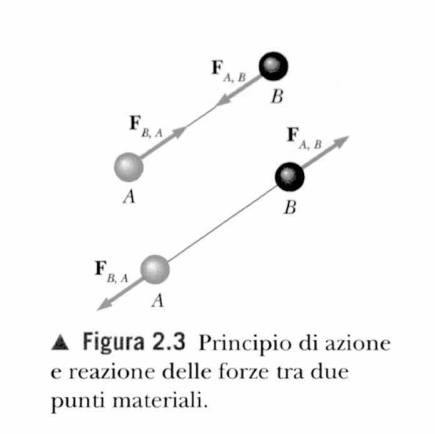
\includegraphics[width=0.5\textwidth]{reazioneazione.png}
\end{minipage}
\begin{minipage}{0.5\textwidth}
    \centering
    \[\bar F_{AB} = -\bar F_{BA}\]
\end{minipage}
\begin{center}
    \textit{Ad ogni azione corrisponde una reazione uguale e contraria.}\\
\end{center}
Se A e B sono la Terra e il sole allora:
\[
    F = G \dfrac{M_t M_s}{r^2} \ \ \ \textit{Gravitazione}
\]
Per le cariche:
\[
    F = k \dfrac{q_1 q_2}{r^2} \ \ \ \textit{Elettromagnetica}
\]
Questo non significa che i due corpi non si muovano, anzi si muovono in qundo il punto di applicazione è diverso: immagina la roulotte e la macchina.
\subsection{Quantità di moto, impulso}
Si definisce quantità di moto di un punto materiale il vettore:
\[
    \bar p = m\bar v
\]
Se la massa è costante la seconda legge di Newton diventa:
\[
    \bar F = \dfrac{d\bar p}{dt}
\]
Da cui si ottiene il teorema dell'impulso:
\[
    \bar F dt = d\bar p \implies \int_{0}^{t_0} \bar F dt = \int_{\bar p_i}^{\bar p_f} d\bar p = \bar p_f - \bar p_i = \Delta\bar p = \bar J
\]
Dove $\bar J$ è l'impulso della forza $\bar F$ e $\Delta p$ è la variazione della quantità di moto. . Il teorema dell'impulso dice che:\\
\textit{l'impulso do una forza applicata a un punto materiale provoca la variazione della quantità di moto}\\
Se la massa è costante:
\[
    \bar F_m \cdot \Delta t = \Delta \bar p \implies \bar F_m = \dfrac{\Delta\bar p}{\Delta t}
\]
\subsubsection{Unità di misura}
\[
    [\bar F] = [M]\cdot\dfrac{[L]}{[T^2]} \implies \dfrac{kg\cdot m}{s^2} = N
\]
\[
    [\bar p] = [M]\cdot\dfrac{[L]}{[T]} \implies \dfrac{kg\cdot m}{s} = N\cdot s
\]
\subsubsection{Esercizio 2.1}
\begin{figure}[H]
    \centering
    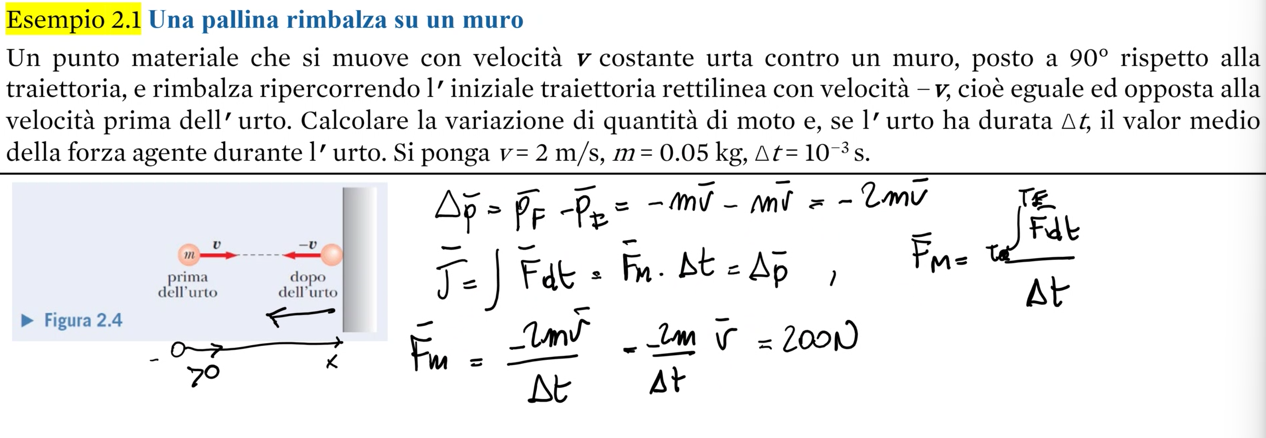
\includegraphics[width=0.7\textwidth]{2-1.png}
\end{figure}

\section{Risultante delle forze, equilibrio}
\begin{minipage}
    {0.5\textwidth}
    \centering
    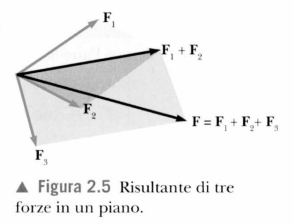
\includegraphics[width=0.5\textwidth]{3forze.png}
\end{minipage}
\begin{minipage}{0.5\textwidth}
    \centering
    Principio di sovrapposizione:\\
    \[
        \bar F = \bar F_1 + \bar F_2 + \bar F_3 + \ldots + \bar F_n = \sum_{i=1}^{n} \bar F_i
    \]
\end{minipage}
e l'accelerazione del punto è pari alla somma vettoriale delle accelerazioni che il punto avrebbe se agisse ciascuna forza separatamente:
\[
    \bar a = \dfrac{\bar F}{m}
\]
\textbf{indipendenza delle azioni simultanee}.\\
Se $\bar F = 0$ e $\bar v = 0$ allora il punto rimane in quiete: sono realizzate le condizioni di equilibrio statico. Devono quindi essere nulle tutte le componenti della risultate ovvero con riferimento a un sistema di assi cartesiani:
\[
    \bar F = \sum_{i} \bar F_i = 0 \implies \begin{cases}
        F_x = \sum_i F_{ix} = 0 \\
        F_y = \sum_i F_{iy} = 0 \\
        F_z = \sum_i F_{iz} = 0
    \end{cases}
\]
\begin{figure}[H]
    \centering
    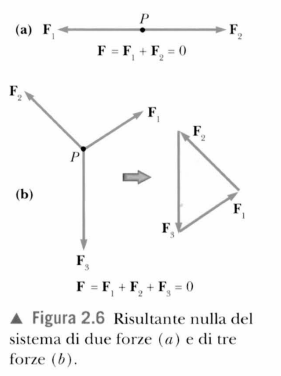
\includegraphics[width=0.3\textwidth]{eq.png}
\end{figure}
\subsubsection{Esercizio 2.2}
\begin{figure}[H]
    \centering
    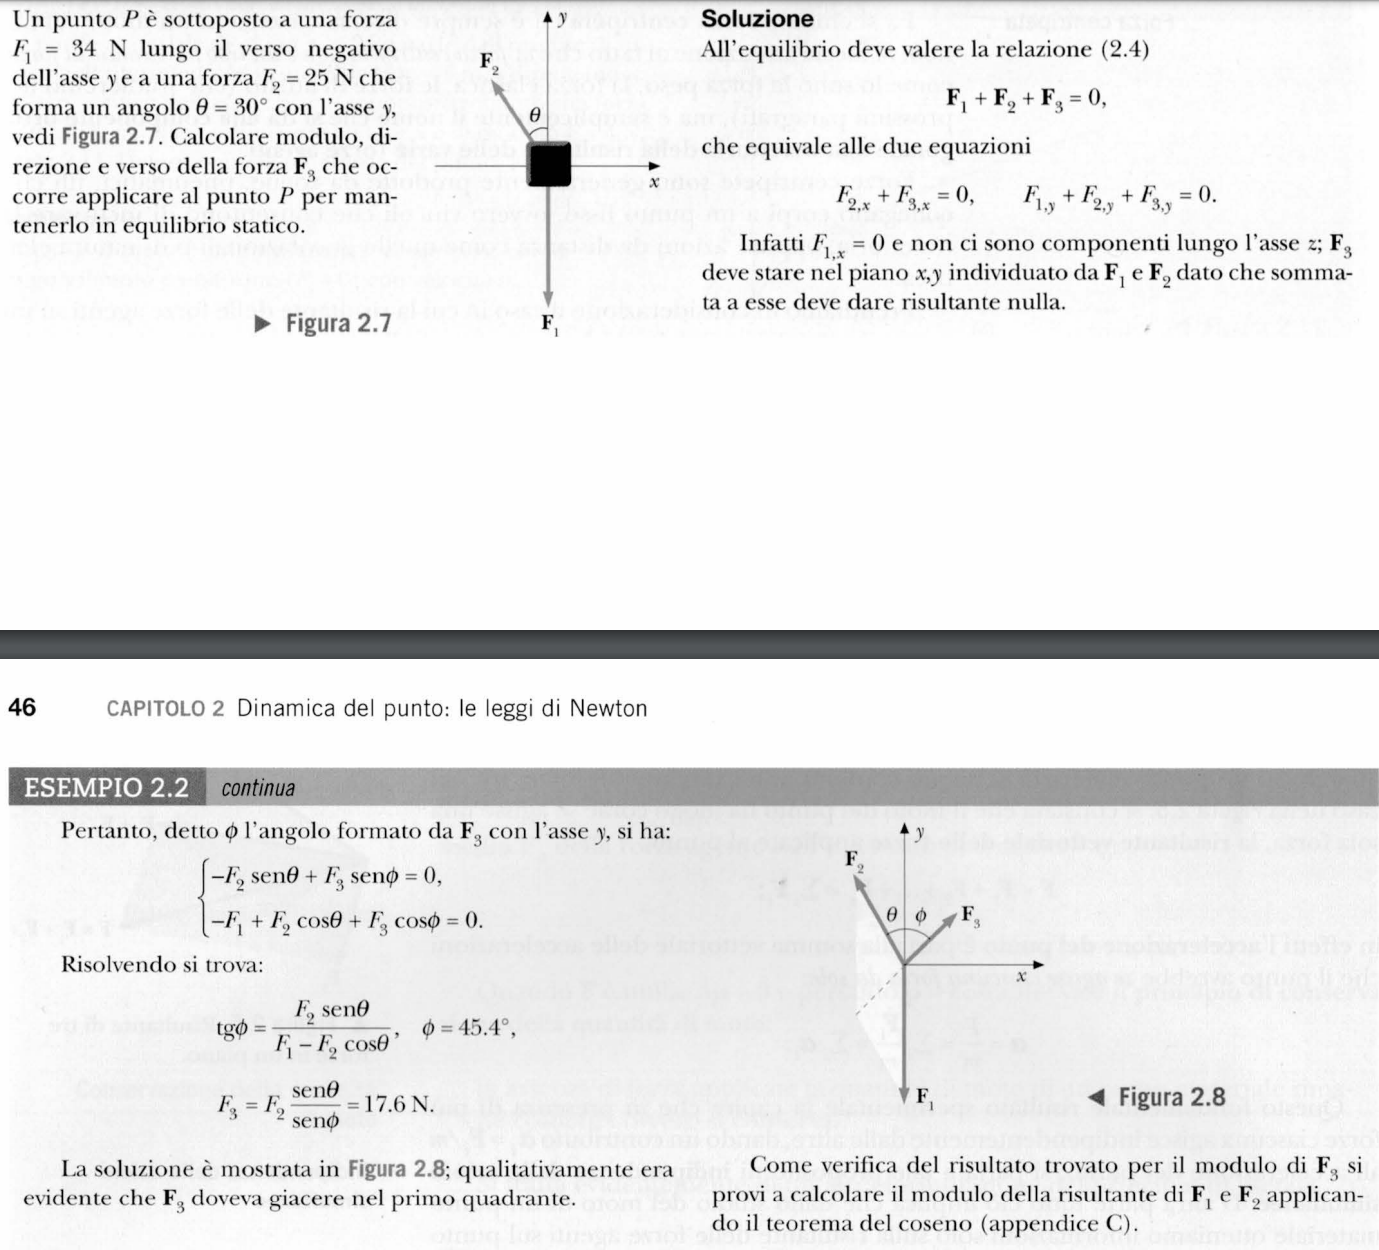
\includegraphics[width=0.7\textwidth]{2-2.png}
\end{figure}


\end{document}